\documentclass[msc,numbers]{coppe}
\usepackage{amsmath,amssymb}
\usepackage{hyperref}
\usepackage{algpseudocode}
\usepackage{algorithm}

\makelosymbols
\makeloabbreviations

\begin{document}
    \title{Change Point Detection in End-to-End Measurements Time Series}
    \foreigntitle{Change Point Detection in End-to-End Measurements Time Series}
    \author{Diego}{Ximenes Mendes}
    \advisor{Prof.}{Edmundo}{Albuquerque de Souza e Silva}{Ph.D.}
  
    %\examiner{Prof.}{Nome do Primeiro Examinador Sobrenome}{D.Sc.}
    %\examiner{Prof.}{Nome do Segundo Examinador Sobrenome}{Ph.D.}
    %\examiner{Prof.}{Nome do Terceiro Examinador Sobrenome}{D.Sc.}
    %\examiner{Prof.}{Nome do Quarto Examinador Sobrenome}{Ph.D.}
    %\examiner{Prof.}{Nome do Quinto Examinador Sobrenome}{Ph.D.}
    \department{PESC}
    \date{01}{2017}
  
    \keyword{Change Point Detection}
    \keyword{Time Series}
    \keyword{Machine Learning}
  
    \maketitle
  
    \frontmatter
    %\dedication{A algu\'em cujo valor \'e digno desta dedicat\'oria.}
  
    %\chapter*{Agradecimentos}
  
    \begin{abstract}
    To better understand the performance of it's own network, a major
Tier-3 Brazilian ISP, in partnership with UFRJ and the startup TGR,
established a project to monitor the service provided to a subset
of it's customers.

In this context, guided by the specific ISP's network's charateristics
and the current measurement process,
this dissertation aims to check the viability of
only using end-to-end QoS measures, and traceroutes,
to identify and localize network events. An event can be interpreted as a
behavioral change in a network equipment, that affect the quality of service
perceived by the end-users,
such as a router failure. The localization procedure defines a set of
feasible locations where the event could have happened.

For such purpose, this work proposes a data analytics framework, which is able
to track statistical changes in the QoS time series of different
clients.
To detect and localize events, the mechanism correlates these modification
patterns with traceroutes.
In order to increase the system's performance,
this dissertation also indicates possible improvements in the current
measurement methodology.

    \end{abstract}
  
    \begin{foreignabstract}
    To better understand the performance of it's own network, a major
Tier-3 Brazilian ISP, in partnership with UFRJ and the startup TGR,
established a project to monitor the service provided to a subset
of it's customers.

In this context, guided by the specific ISP's network's charateristics
and the current measurement process,
this dissertation aims to check the viability of
only using end-to-end QoS measures, and traceroutes,
to identify and localize network events. An event can be interpreted as a
behavioral change in a network equipment, that affect the quality of service
perceived by the end-users,
such as a router failure. The localization procedure defines a set of
feasible locations where the event could have happened.

For such purpose, this work proposes a data analytics framework, which is able
to track statistical changes in the QoS time series of different
clients.
To detect and localize events, the mechanism correlates these modification
patterns with traceroutes.
In order to increase the system's performance,
this dissertation also indicates possible improvements in the current
measurement methodology.

    \end{foreignabstract}
  
    \tableofcontents
    \listoffigures
    \listoftables
    \printlosymbols
    \printloabbreviations
  
    \mainmatter
  
    \chapter{Introduction}

To better understand the performance of it's own network, a major
tier-3 Brazilian \gls*{isp}, in partnership with \gls*{ufrj} and a startup
incubated at this university,
established a project to monitor the service provided to a subset
of it's customers.

Considering the \gls*{isp}'s cable-television infrastructure,
which runs \gls*{docsis},
\gls*{qos} metrics are gathered through a software placed at home routers
connected to cable modems. This software is responsible to perform end-to-end
measurements against servers strategically located by the \gls*{isp}.

In this context, guided by the specific \gls*{isp}'s network's characteristics,
and the current measurement process,
this dissertation aims to check the viability of
only using end-to-end \gls*{qos} measures, and traceroutes,
to identify and localize network events. An event can be interpreted as a
behavioral change in a network equipment, that affect the quality of service
perceived by the end-users,
such as a router failure. The localization procedure defines a set of
feasible locations where the event could have happened.

For such purpose, this work proposes a data analytics framework, which is able
to track statistical changes in the \gls*{qos} time series of different
clients.
To detect and localize events, the mechanism correlates these modification
patterns with traceroutes.
In order to increase the system's performance,
this dissertation also indicates possible improvements in the current
measurement methodology.

\section{Contributions}

Considering the specific \gls*{isp}'s network topology,
and the already implemented
measurement process, next is listed this dissertation's main contributions.

\begin{itemize}
\item
A data analytics procedure, that only uses the available end-to-end \gls*{qos}
measurements, and traceroutes, to detect and localize network events.

\item
A list of possible improvements in the measurement methodology currently
employed by the startup, in order to enhance the proposed system's performance.

\end{itemize}

\section{Dissertation Outline}

Chapter~\ref{chap:literature_review} consists of a literature review, that
describes three previous systems that use
end-to-end measurements to localize network events.
To track statistical changes in the time series, the current
work deploys change point detection methods. Then,
Chapter~\ref{chap:change_point_detection} presents several of these algorithms,
including the developed strategies to better handle the end-to-end \gls*{qos} data
characteristics.
In Chapter~\ref{chap:methodology} is detailed the measurement methodology and
the proposed data analytics workflow.
Chapter~\ref{chap:results} presents several results when the proposed pipeline
was applied to real data.
Finally, Chapter~\ref{chap:conclusion} concludes the work and
points future directions.

The code developed to support this dissertation is available at
\url{https://bitbucket.org/diegoximenes/master_thesis}.
Unfortunately, due to a \gls*{nda},
the data used in this project can not be open sourced.

    \chapter{Change Point Detection} 

A change point detection algorithm is concerned to identify points in time where the statistical properties of a time series have changed. This problem have a broad application in different knowledge fields, and in general, the algorithms performance are closely related with the input characteristics. Also, if the latent information of the procedures that generated a time series is missing, the target statistical properties can be considered subjective, bringing difficulties not only in the detection phase but also in the problem formalization.

In this context this chapter specifies the problem and briefly discusses several change point detection algorithms. The literature of this area is extensive, and it is common to find methods that presents a poor performance due to a variety of reasons, such as they are too specific or because the mechanisms were only analyzed through theoretical aspects. Therefore, it was chosen a set of methods that can provide a good practical and theoretical perspective, and also flexibility to insert adaptations that can better handle some input peculiarities. Furthermore, through this chapter is exposed several obstacles when dealing with real data, and some adopted solutions which are not described in literature.

\section{Problem Definition}

The problem can be categorized in offline or online. In the offline version, to decide if a specific point at time $t$ is a change point the solver has available the whole time series, including past and future information on $t$. In the other hand, in the online version the information is available up to time $t$. The choice between these options is defined by the application domain, in some cases data are processed in real time and the change points should be detected as soon as possible, but in others the changes are identified by historical purposes and offline algorithms can be used. 

It is intuitive that the offline case is more robust, since there are more information to make a classification. In practice, to increase the statistical confidence of a decision the online definition is relaxed, and to decide if a point at time $t$ is a change point it is possible to use data up to a small window in the future of $t$, which in real time processing means that the application should wait until more data are available. This trick plays a trade-off between minimizing the time to detect a change and correctly classify a point. Therefore, in some cases, the online version can be transformed in the offline case by only modifying the input availability. 

In this work it is considered the following input and change points characteristics, which were defined considering the final application scenario:
\begin{itemize}
    \item Univariate time series. However, it is possible to extend several methods presented here to deal with multivariate data.
    \item Unevenly time series, that is, data is not regularly sampled in time.
    \item Time series with different lengths.
    \item Unknown number of change points.
    \item Different number of points between change points.
    \item Focus on changes in the underlying mean and distribution, disregarding other kinds of changes such as in periodicity.
    \item Outliers are not considered statistical changes.
    \item There is no latent information of the time series.
    \item It is considered the online and offline options.
\end{itemize}

\section{Notation}

An univariate time series composed of $n$ points is defined by two vectors, $\mathbf{x} = (x_{1}, ..., x_{n})$ and $\mathbf{y} = (y_{1}, ..., y_{n})$. The value $y_{i}$ indicates the $i$-th sampled value and $x_{i}$ indicates the associated sample time. It is assumed that the points are sorted by time, that is, $x_{i - 1} < x_{i}$ for $i = 2, ..., n$. Since unevenly time series is considered, $x_{i} - x_{i - 1}$ can be different for different $i$ values. For $s \ge t$ the following convention is adopted: $\mathbf{y}_{s:t} = (y_{s}, ..., y_{t})$.

The presence of $k$ change points implies that data is split into $k+1$ segments, also called windows. Let $\tau_{i}$ indicates the $i$-th change point for $i=1,...,k$. Also let $\tau_{0} = 0$, $\tau_{k + 1} = n$ and $\boldsymbol \tau = (\tau_{0}, ..., \tau_{k + 1})$. Then, the $i$-th segment is defined by $\mathbf{y}_{\tau_{i - 1} + 1 : \tau_{i}}$, assuming that $\tau_{i - 1} < \tau_{i}$ for $i = 1, ..., k + 1$.

Through the previous definitions, change point detection algorithms mainly aim to find both $k$ and $\boldsymbol \tau$.

\section{Sliding Windows}

Sliding windows techniques use two sliding windows over the time series, and reduce the problem of detecting change points to the problem of testing whether data from the segments were generated by different distributions. One approach is to consider a distance metric between two empirical distributions as the base to infer the change points. Letting $d(\mathbf{a}, \mathbf{b})$ be the distance between two empirical distributions defined by the windows $\mathbf{a}$ and $\mathbf{b}$, and considering windows of length $m$, the Algorithm~\ref{alg:sliding_windows} presents a simple sliding windows method.

\begin{algorithm}
    \caption{Sliding Windows}
    \label{alg:sliding_windows}
	\begin{algorithmic}[1]
		\State $i \gets 1$
		\While{$i + 2 m - 1 \leq n$}
             \If{$d(\mathbf{y}_{i : i + m - 1}, \mathbf{y}_{i + m : i + 2m - 1}) > \alpha$}
                \State Report $i + m - 1$ as a change point
		        \State $i \gets i + m$
             \Else
		        \State $i \gets i + 1$
             \EndIf
        \EndWhile
	\end{algorithmic}
\end{algorithm}

In this method, when the distance between the distributions is above some threshold $\alpha$ a change point is reported. This is a common approach for an online application, however, it is possible to increase the classification accuracy in offline cases. As an example, the top plot of figure~\ref{fig:sliding_window_toy_example} presents a simulated time series, the segment $\mathbf{y}_{1 : 1000}$ was generated sampling a $N(1, 0.2)$ distribution, and $\mathbf{y}_{1001 : 2000}$ was sampled through $N(5, 0.2)$. The distribution of a window was constructed binning the data with bins of size 0.02. The bottom plot of the same figure presents the associated Hellinger distance \cite{hellinger_distance} between two sliding windows, where the point $(i, H_{i})$ represents the distance between the windows $\mathbf{y}_{i - 100 : i - 1}$ and $\mathbf{y}_{i : i + 99}$.

\begin{figure}[H]
    \centering
    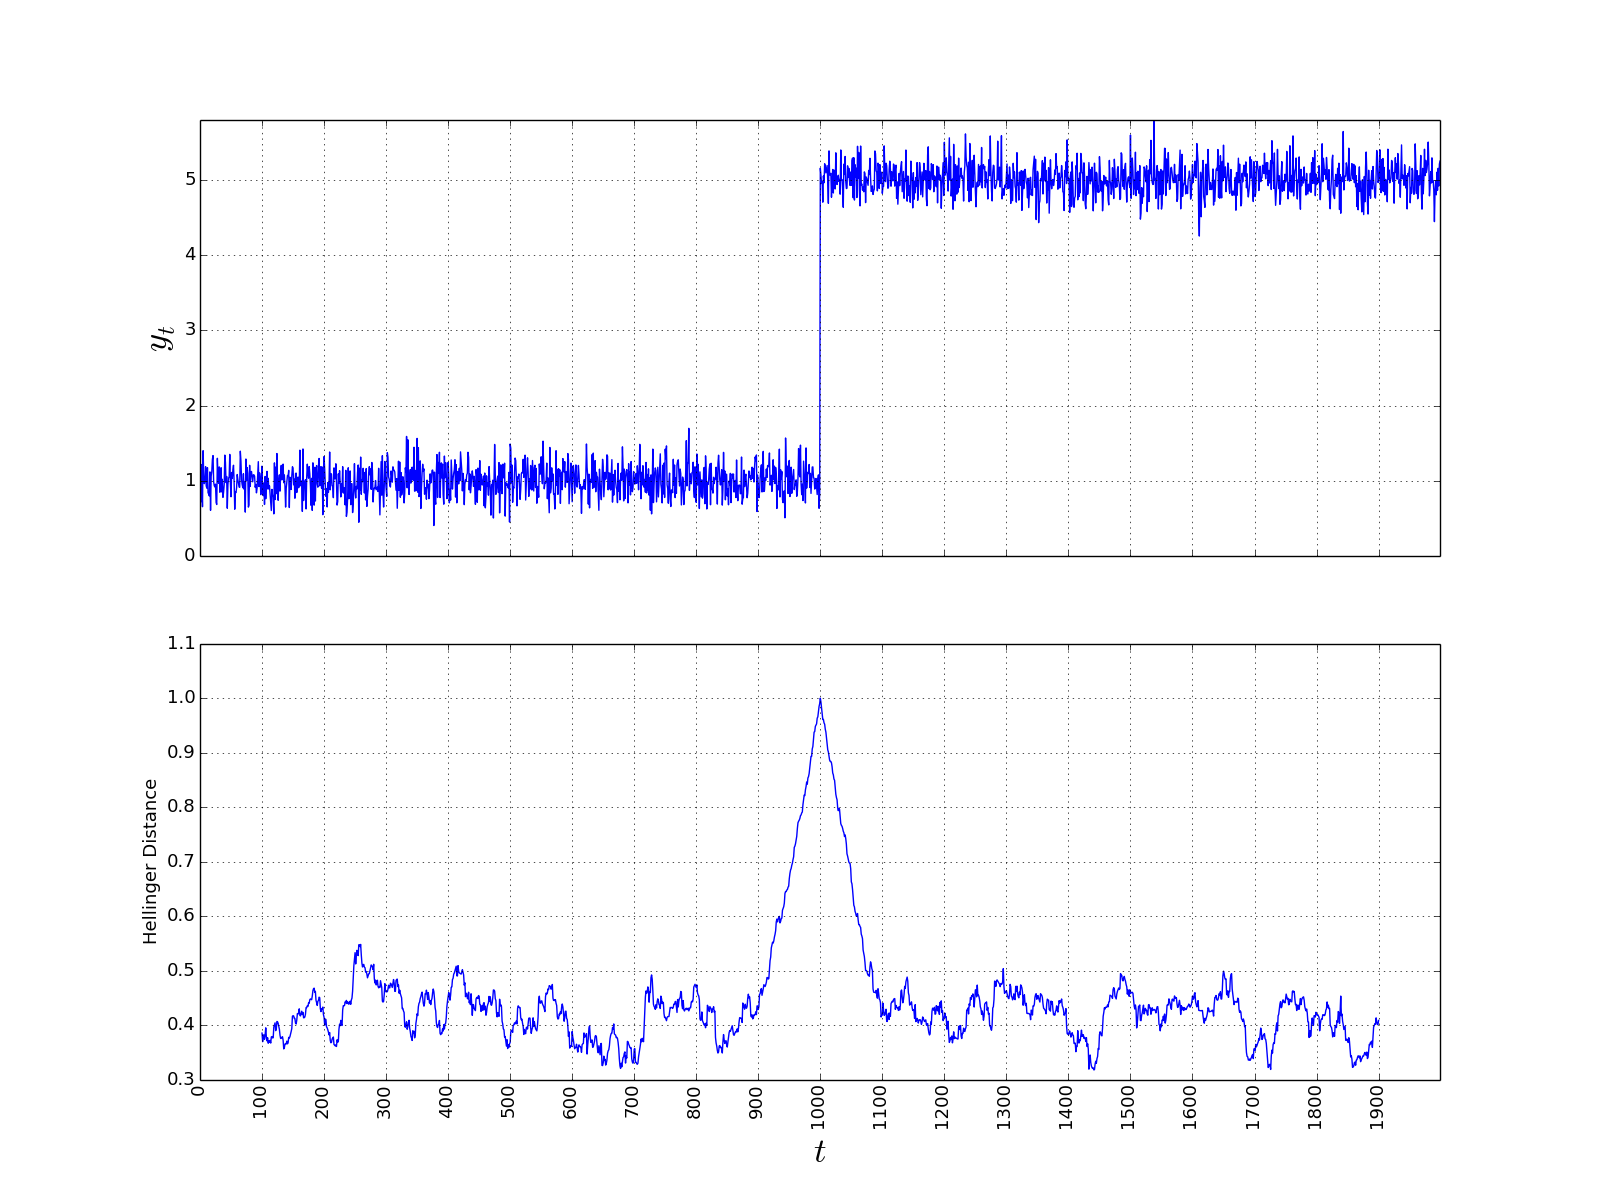
\includegraphics[width=1.0\textwidth]{./figures/sliding_window_toy_example.png}
    \caption{Toy example of a sliding windows method.}
    \label{fig:sliding_window_toy_example}
\end{figure}

It can be observed that there is a peak on the distance in the exact location where the distribution changed. However, using only the threshold method it is possible to prematurely infer the position of the change point, therefore, an alternative is to also use a peak detection algorithm. Besides, the distance function choice has a direct impact on the classification accuracy.

As stated in \cite{detecting_change_in_data_streams}, a performance improvement can be achieved concurrently executing the same sliding windows algorithm, however, with different windows lengths, which facilitates the detection of segments with distinct number of points.

\section{Optimization Model}  

Given a fixed value of $k$, one approach is to define a cost function that measures the homogeneity of a window, and therefore, choose the change points that globally optimize this homogeneity. Let the cost of the $i$-th segment be defined as $C(\mathbf{y}_{\tau_{i - 1} + 1 : \tau_{i}})$, then the cost of a segmentation is the sum of all segments costs.

A common choice for the function $C$ is the MSE (Mean Squared Error), which can capture changes in the mean. Another usual approach is to consider distribution changes through negative maximum log-likelihood functions, considering that data within a window is iid. 

Therefore, given a fixed $k$, the optimal segmentation is obtained through the following optimization problem, which is called the constrained case \cite{on_optimal_multiple_changepoint_algorithms_for_large_data}: 

\begin{equation}
    \min_{\boldsymbol \tau_{1 : k}} \sum \limits_{i = 1}^{k + 1} C(\mathbf{y}_{\tau_{i - 1} + 1 : \tau_{i}})
\end{equation}

This problem can be solved using dynamic programming with $O(k n^2 f(n))$ time complexity, where $f(n)$ is related with $C$ evaluation. Several segment cost functions can be evaluated in $O(1)$ after a $O(n)$ preprocessing phase, implying in an overall $O(k n^2)$ complexity. It is possible to proof that MSE, negative maximum log-likelihood functions of normal, exponential, poisson and binomial distributions have this characteristic. Also, the formulation can consider a minimum value of a window length.

Modeling segments with continuous distributions can lead to practical difficulties. One of them is the fact that segments can form degenerate distributions, that is, the data of a window can have zero variance, which is always the case of unitary length segments. In these scenarios the negative maximum log-likelihood is undefined. Two approaches can be used to overcome this situation. The first one tries to avoid degenerate segments adding a white noise with small variance to the time series. The second one considers that the cost of any degenerate distribution is equal to a constant.


% Using discrete distributions it is possible to easily compare direct compare the likelihood of two different distribution types. 

% Since the likelihood of different continuous distributions can`t be directly compared, is not possible to apply the segmentation algorithm considering different types of continuos distributions. One possibility to handle this is to apply automatic methods to check which kind of distribution fits better to the segment, such as Kolmogorov-Smirnov. This was not approached in this work due to the computation time efficiency decrease and that since we deal with small number of data possibly these methods would have a poor performance.

When the number of change points is unknown an usual way is to introduce a non decreasing penalty function $g(k)$. Then, the new optimization problem, called penalized case \cite{on_optimal_multiple_changepoint_algorithms_for_large_data}, is:

\begin{equation}
    \min_{k, \boldsymbol \tau_{1 : k}} \sum \limits_{i = 1}^{k + 1} C(\mathbf{y}_{\tau_{i - 1} + 1 : \tau_{i}}) + g(k)
\end{equation}

This problem can be solved in $O(K n^{2} f(n))$. However, if the penalty function is linear in $k$, the problem can be formulated more efficiently and solved in $O(n^{2} f(n))$.

Also, there are several pruning algorithms to speedup the computation \cite{optimal_detection_of_changepoints_with_a_linear_computational_cost, on_optimal_multiple_changepoint_algorithms_for_large_data, computationally_efficient_changepoint_detection_for_a_range_of_penalties}, in general trying to reduce the $\boldsymbol \tau$ search space but maintaining optimality.

\section{HMM (Hidden Markov Model)}

The idea that each segment is associated with a specific latent configuration has a direct interpretation to a HMM model \cite{a_hidden_markov_model_segmentation_procedure_for_hydrological_and_environmental_time_series, fast_estimation_of_posterior_probabilities_in_change-point_analysis_through_a_constrained_hidden_markov_model, inertial_hidden_markov_models_modeling_change_in_multivariate_time_series}. In this context, each window is related to a hidden state of a HMM, and the observation distribution of this state represents the distribution of that segment. Therefore, the mechanism models the time series using a HMM, and through the hidden state path assesses the times when a transition between different hidden states occur.

There are several approaches in the detection and training phases. For example, given a trained HMM, is possible to analyze the most probable hidden state path that a time series can follow through the viterbi algorithm. Also, it is possible to evaluate the probability of a transition between different hidden states at time $t$, and then apply a threshold and peak detection methods, as well as in sliding windows techniques. For the training step, it is possible to use several time series to train a single HMM, and then use this model to detect change points in all time series. Another way is to, for each time series, train a single model using only the target time series.

It is important to note that the structure of the hidden state graph has a large impact on the performance. Using a fully connected graph, the number of states defines the maximum number of distribution configurations. Employing a left to right structure, the number of hidden states will induce the maximum number of segments.

In \cite{inertial_hidden_markov_models_modeling_change_in_multivariate_time_series} is stated that when using a fully connected structure, the time interval that a time series stays in the same hidden state is low, which can not reflect real data. To overcome this problem, \cite{inertial_hidden_markov_models_modeling_change_in_multivariate_time_series} suggests to increase the time that a time series stands in the same hidden state, using a dirichlet prior regularization.

\section{Bayesian Inference}

There are several Bayesian methods with the objective to assess the probability that a point is a change point. Following an offline fashion, the work of \cite{exact_and_efficient_bayesian_inference_for_multiple_changepoint_problems} recursively calculates, for each $i$, the probability of $\mathbf{y}_{i : n}$ given a change point at $i$. With these probabilities is possible to simulate the time of the first change point, and then, compute the conditional distribution of the time of the second change given the first, and so on. To achieve this, the mechanism assumes that observations are independents, and that each segment is modeled by conjugate priors. Also, the procedure considers priors to model the number of changes and the time between two consecutive change points. The overall complexity of this method is $O(n^{2})$, considering that the likelihood of a segment can be evaluated in $O(1)$.

In \cite{bayesian_online_changepoint_detection} it is also considered that parameters of different segments are independents, and that data within a window is iid. However, through an online mode, the procedure is concerned with the estimation of the distribution of the length of the current time since the last change point, called run length, given the data so far observed. To achieve this, the method assumes the probability of current run length given the last run length as a prior. Assuming exponential-family likelihoods to model a segment, the time complexity to process a point is linear in the number of points already observed. 

    \chapter{Dataset}

This chapter describes the used datasets, presenting their construction methodology and a brief descriptive analysis.

\section{End-to-End Packet Loss Fraction Time Series Dataset}

\subsection{Methodology}

The time series presented in this work represent network end-to-end measures of a cable-television infrastructure running DOCSIS, with asymmetric download and upload bandwidths. The measurement infrastructure consists of home routers connected to the cable modem, that run a software developed by TGR in partnership with UFRJ. In this is way is possible to measure several metrics, such as link throughput, round trip latency, loss rates, among others. Each home router communicates with one or more servers devoted to execute the different measurement protocols and to store data. Measurement values from each home router are consolidated twice per hour and, by the end of every day, they are transferred to a database for analysis. The servers are strategically located by the ISP and, since the same home router can connect to more than one server, metrics from the same client to different servers can be contrasted. The resulted time series are unevenly due to a variate of reasons. One of them is that measurements are initiated only if the residential link is not under use by the ISP customer, another one is that the home router can be without Internet access or even eletrical energy.

The focus of this work is to analyze the loss fraction, however, \cite{a_preliminary_performance_measurement_study_of_residential_broadband_services_in_brazil} presents a further analysis on other metrics. Round trip packet loss fraction between the home router and the associated server is obtained by sending a train of short UDP packets by the home router and bounced back by the server. The interval between two packets in a train is configurable as well as the length of the train. The data presented in this work considers a train of 100 UDP packets of 32 bytes in which packets are 1 milliseconds apart.

\subsection{Descriptive Analysis}

The TGR software run in a subset of the ISP customers in several brazilian states. In the analysis of this section, was analysed the period from 01 may 2016 to 20 may 2016. Were selected every home router that measured at least one time and that all measures occurred to same server which necessaryly belonged to the same ufs. This filter resulted in 1870 clients time series and 1537272 measures.

In figure~\ref{fig:cdf_ccdf} is presented the packet loss CDF of all time series. It is possible to note that 93.2\% of the measures have zero losses.

\begin{figure}[H]
    \makebox[\linewidth][c]
    {
        %
        \centering
        \begin{subfigure}[b]{0.55\textwidth}
            \centering
            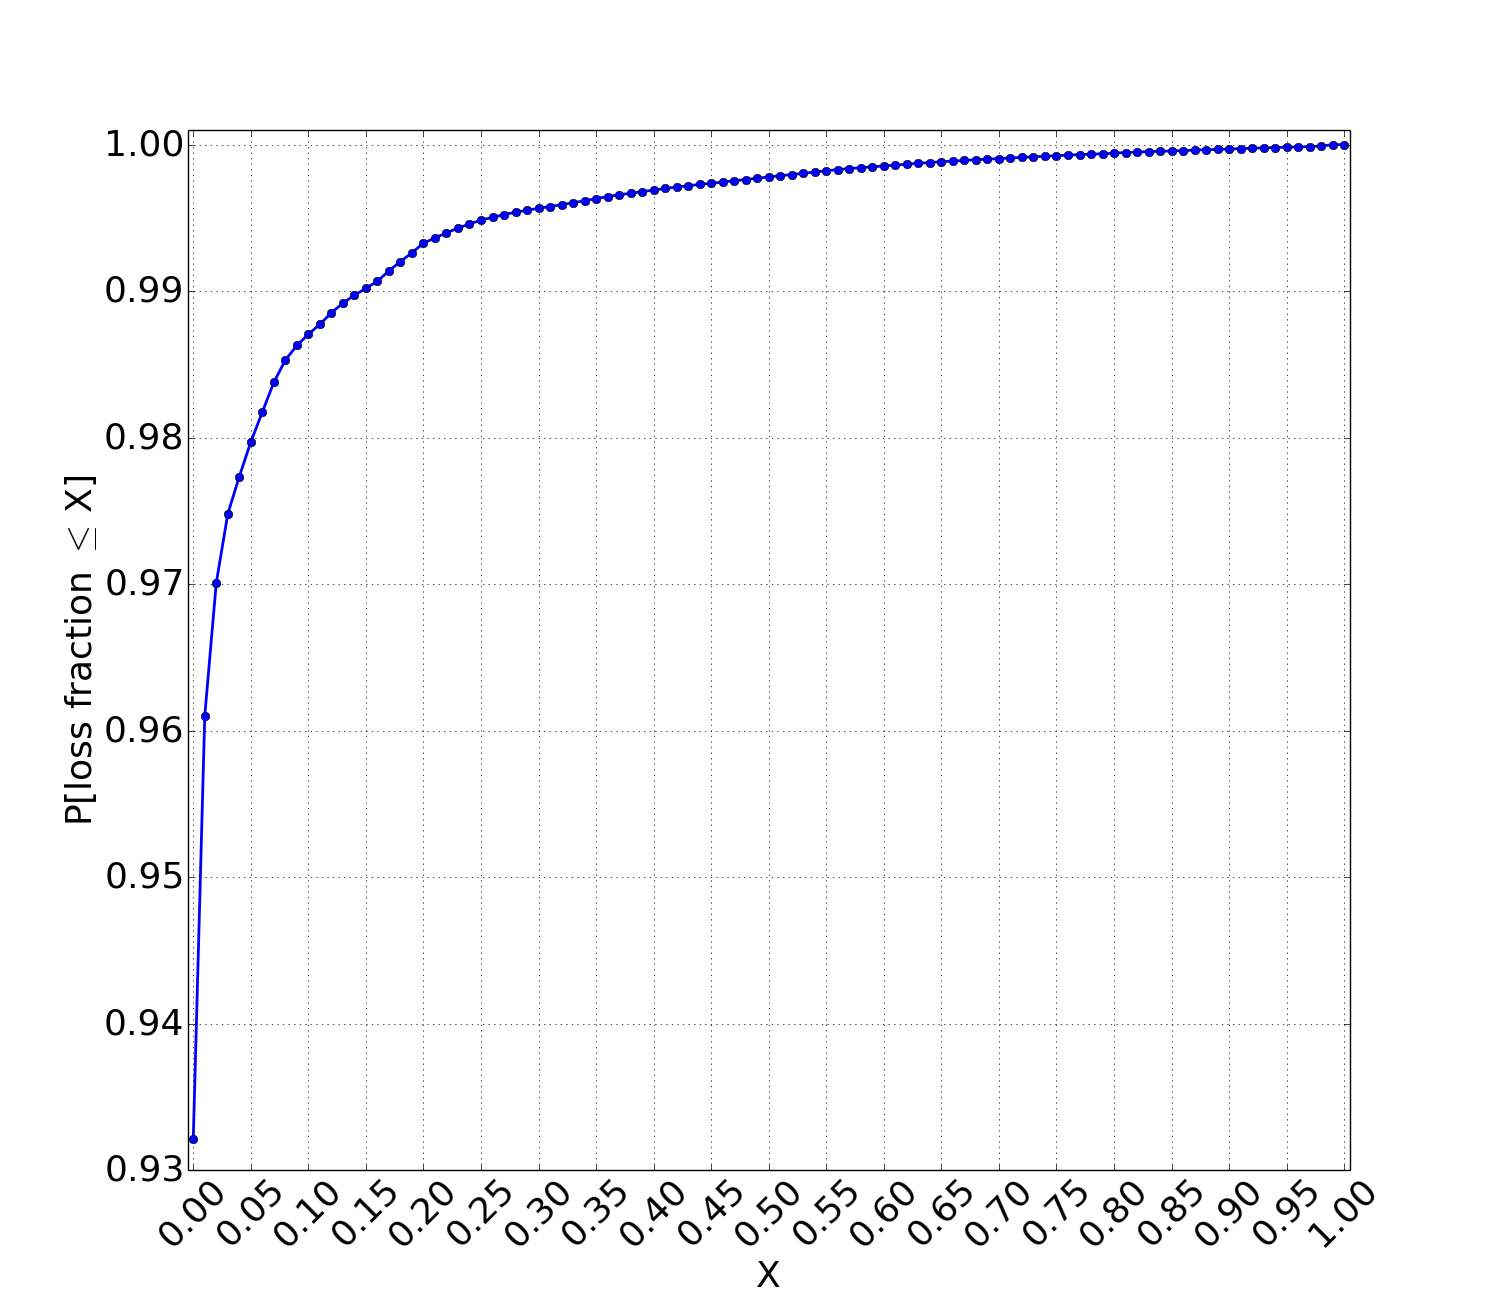
\includegraphics[width=\linewidth]{./figures/loss_cdf.png}
            \caption{CDF}
        \end{subfigure}%
        ~ 
        \begin{subfigure}[b]{0.55\textwidth}
            \centering
            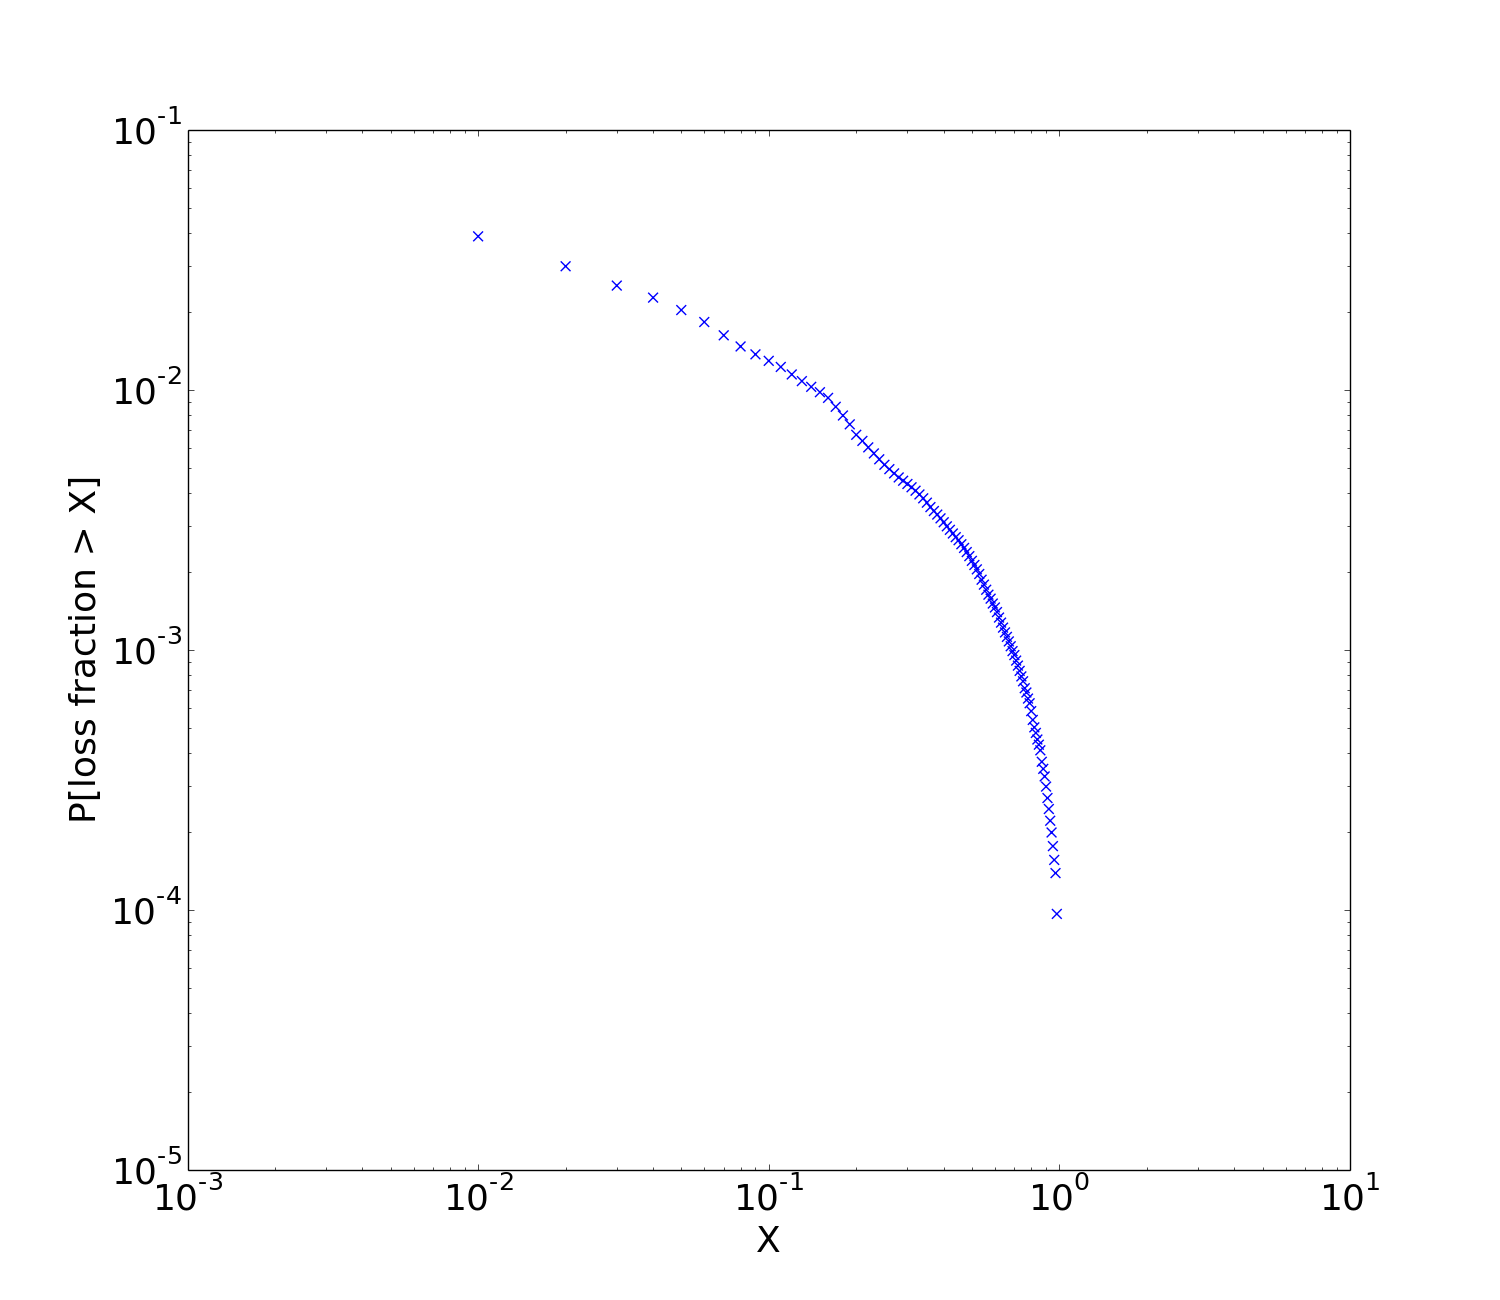
\includegraphics[width=\linewidth]{./figures/ccdf.png}
            \caption{CCDF}
        \end{subfigure}
    }
    \caption{Packet Loss Fraction}
    \label{fig:cdf_ccdf}
\end{figure}%

Figures \ref{fig:acf_ts_1}, \ref{fig:acf_ts_2}, \ref{fig:acf_ts_3} show three examples with common autocorrelation patterns in this dataset together with the time series. Since the time series are unenvely, to compute the autocorrelation function, the raw time series is transformed, and it is only considered the date and hour of a measure, ignoring the minutes and seconds. Therefore, if more than one measure occurs in the same hour, it is considered the mean.

\begin{figure}[H]
    \makebox[\linewidth][c]
    {
        %
        \centering
        \begin{subfigure}[b]{0.55\textwidth}
            \centering
            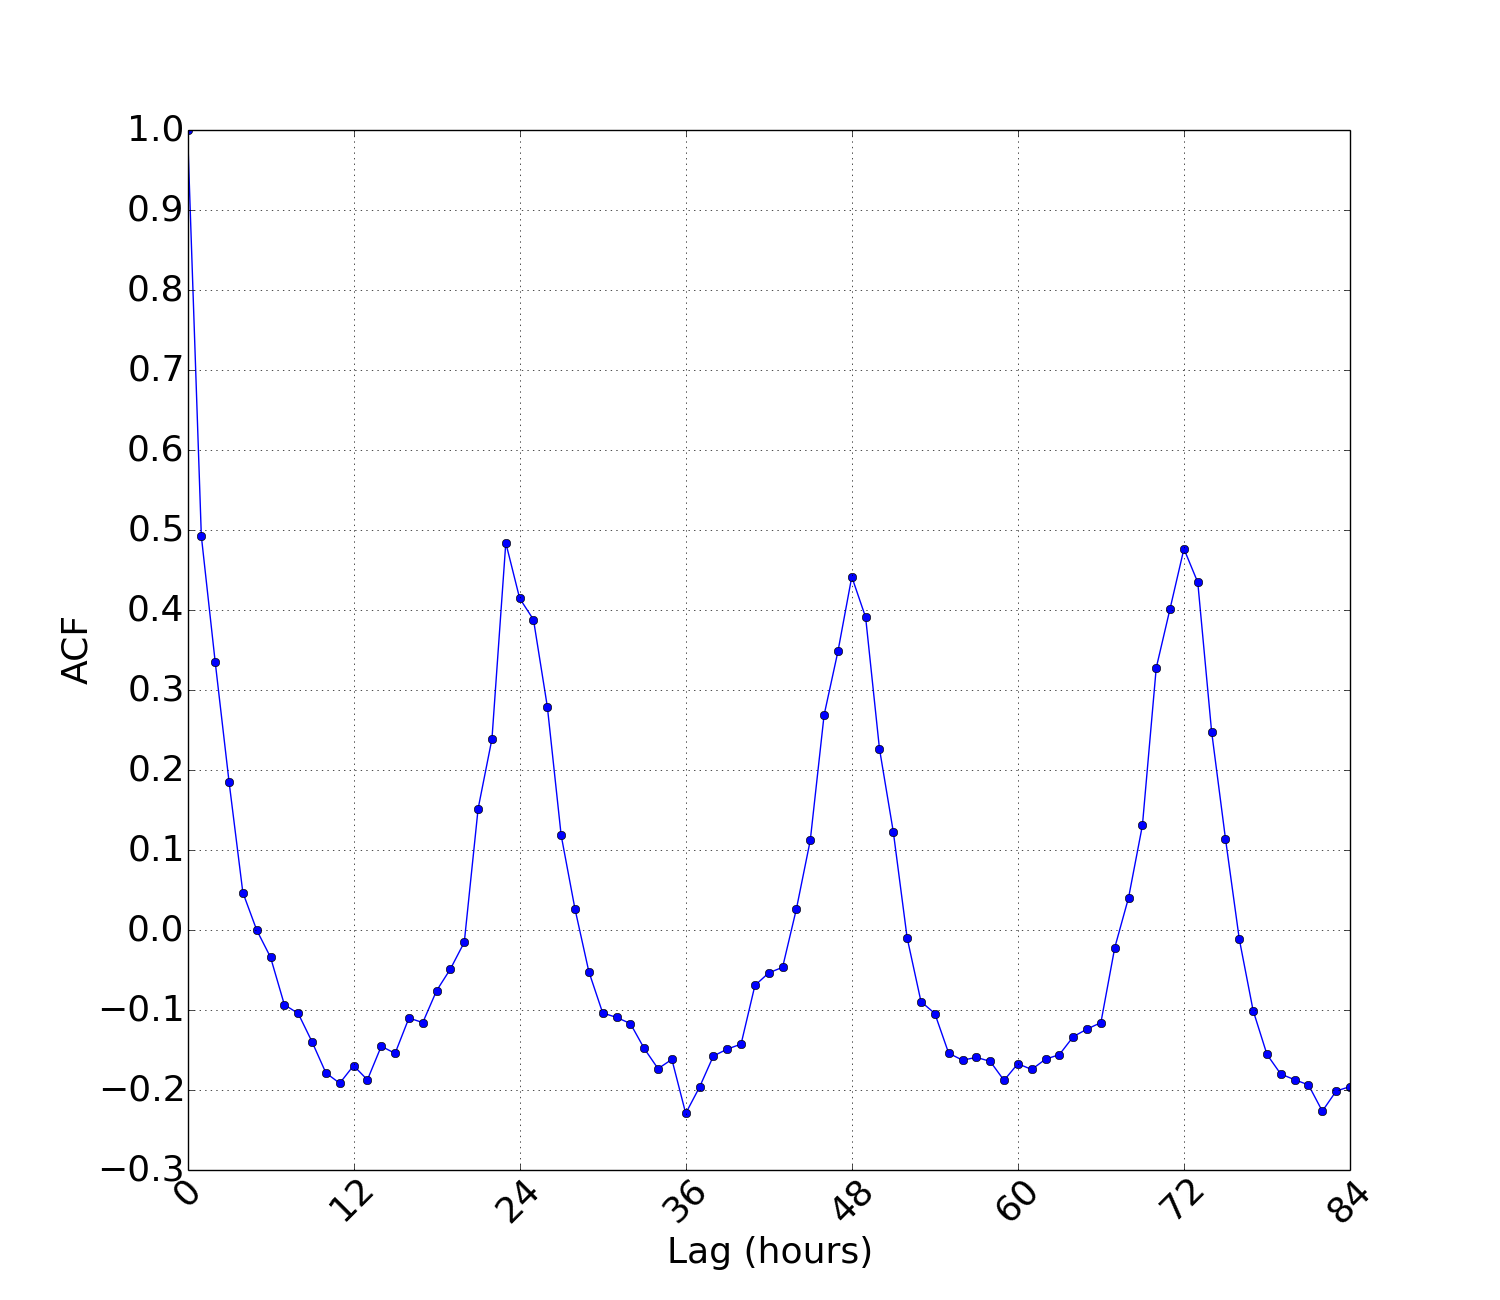
\includegraphics[width=\linewidth]{./figures/acf_NHODTCSRV04_64:66:B3:50:05:BC.png}
            \caption{Autocorrelation}
        \end{subfigure}%
        ~ 
        \begin{subfigure}[b]{0.55\textwidth}
            \centering
            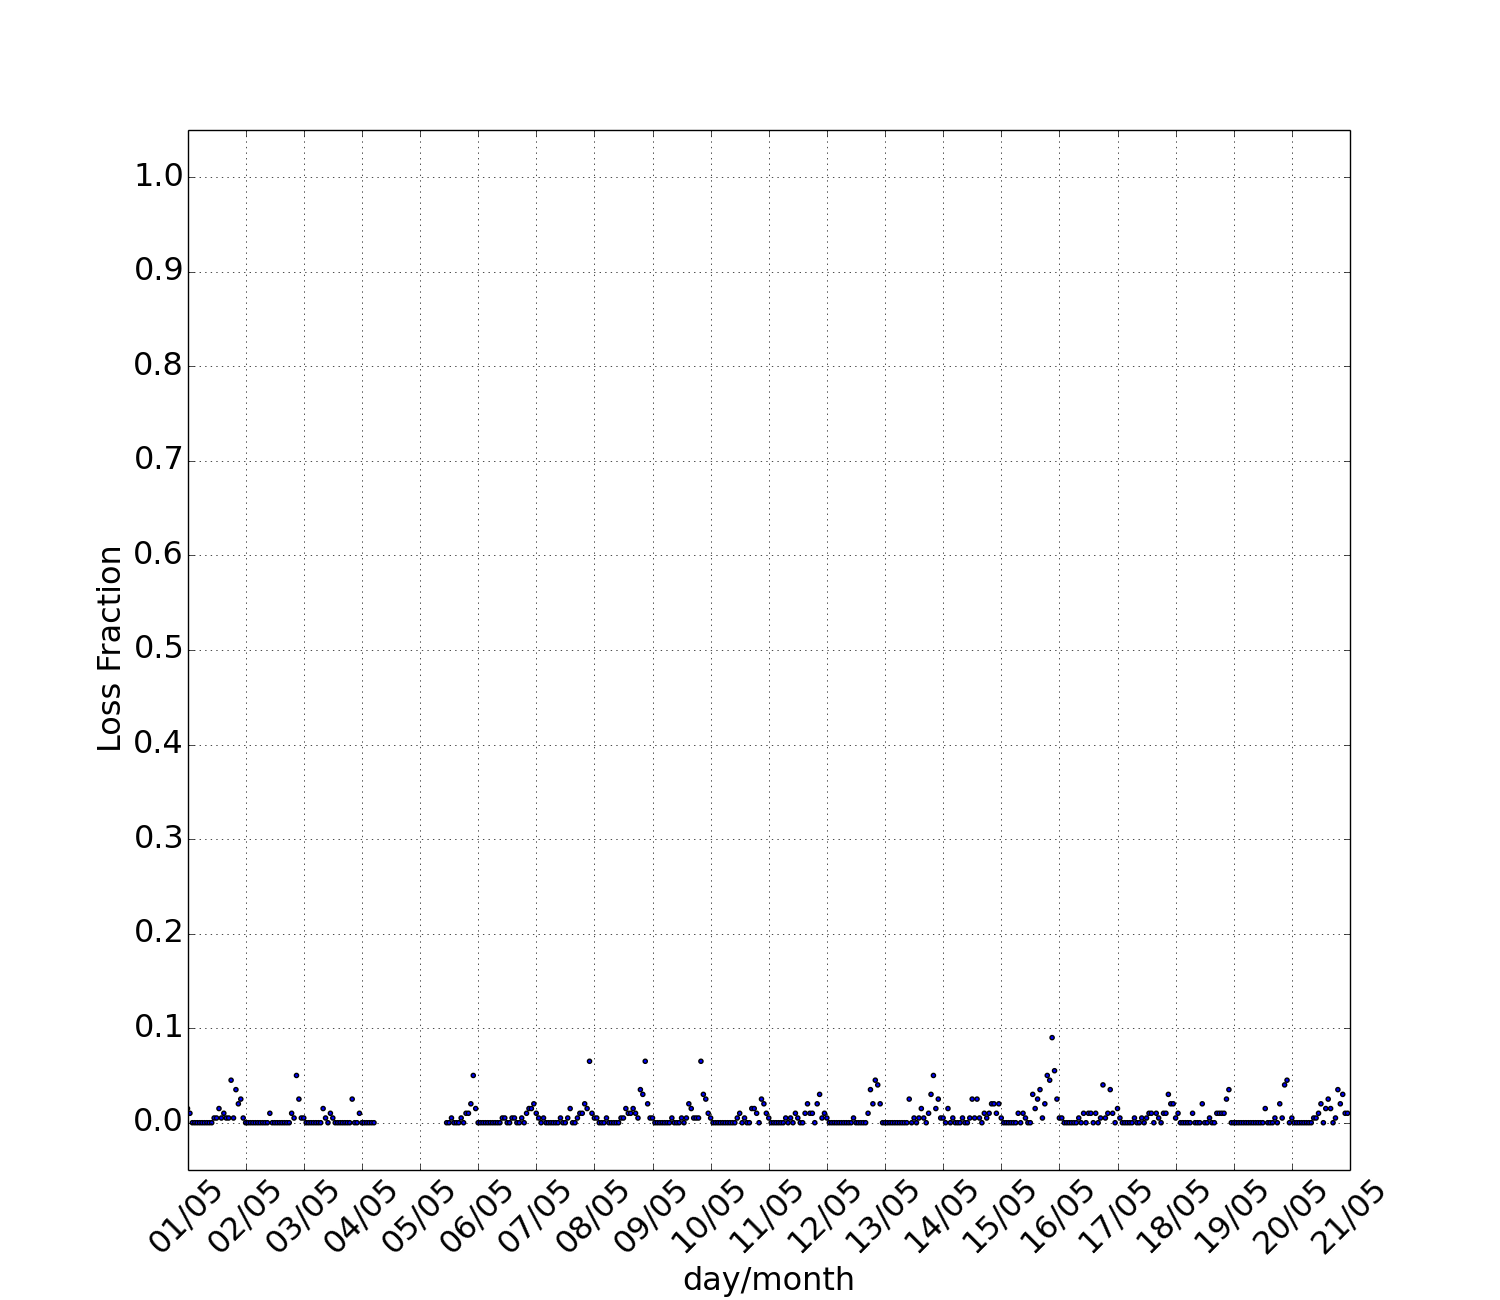
\includegraphics[width=\linewidth]{./figures/ts_NHODTCSRV04_64:66:B3:50:05:BC.png}
            \caption{Time Series}
        \end{subfigure}
    }
    \caption{Client 1}
    \label{fig:acf_ts_1}
\end{figure}%

\begin{figure}[H]
    \makebox[\linewidth][c]
    {
        %
        \centering
        \begin{subfigure}[b]{0.55\textwidth}
            \centering
            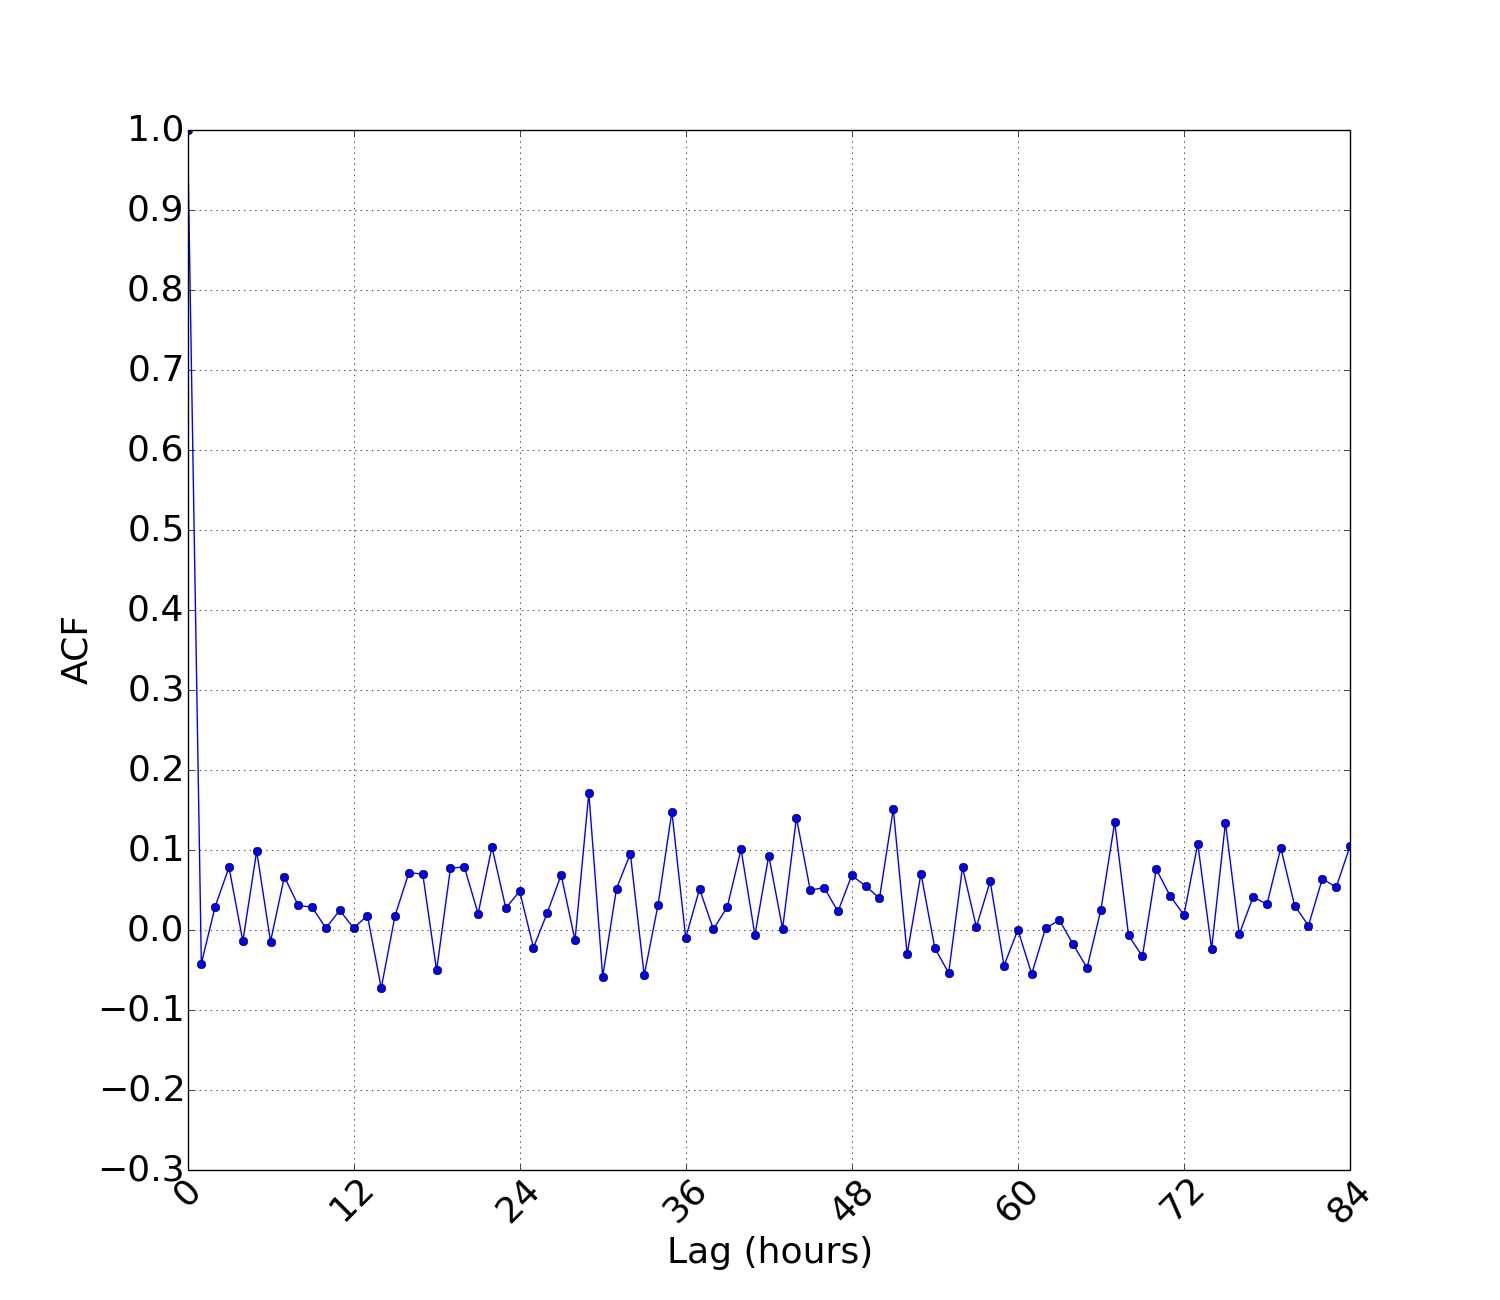
\includegraphics[width=1.0\textwidth]{./figures/acf_BREDTCSRV20_64:66:B3:7B:9E:6A.png}
            \caption{Autocorrelation}
        \end{subfigure}%
        ~ 
        \begin{subfigure}[b]{0.55\textwidth}
            \centering
            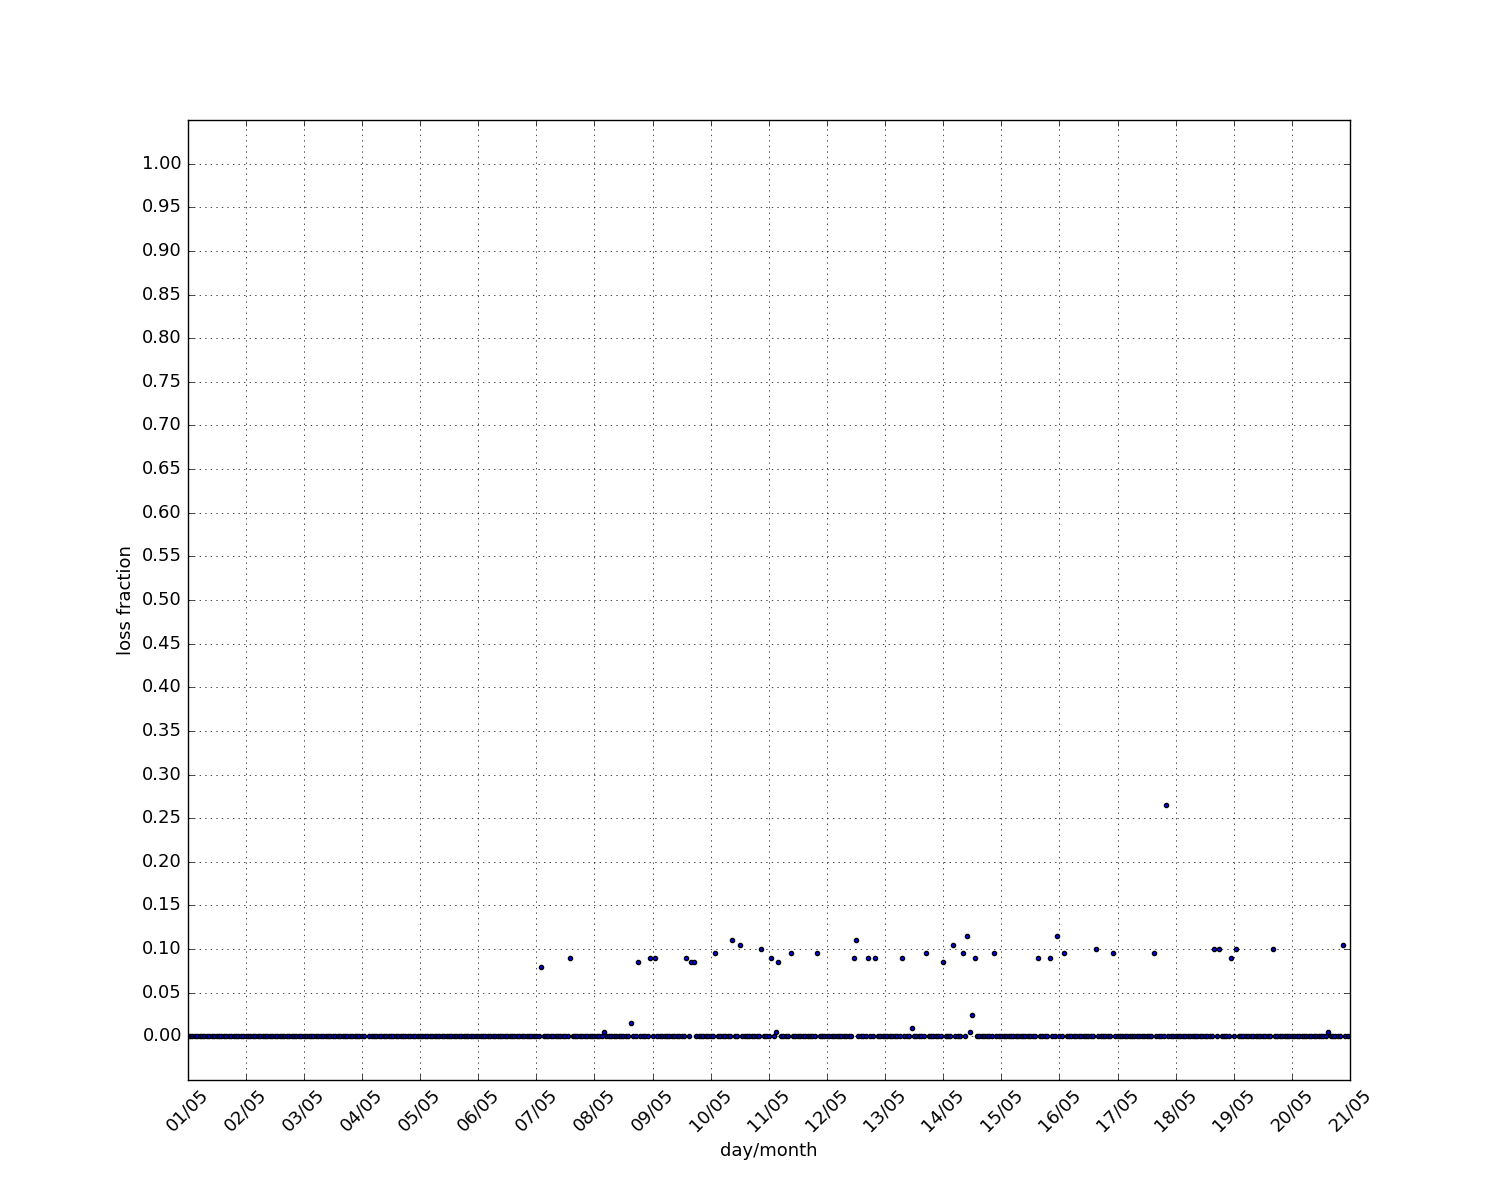
\includegraphics[width=1.0\textwidth]{./figures/ts_BREDTCSRV20_64:66:B3:7B:9E:6A.png}
            \caption{Time Series}
        \end{subfigure}
    }
    \caption{Client 2}
    \label{fig:acf_ts_2}
\end{figure}

\begin{figure}[H]
    \makebox[\linewidth][c]
    {
        %
        \centering
        \begin{subfigure}[b]{0.55\textwidth}
            \centering
            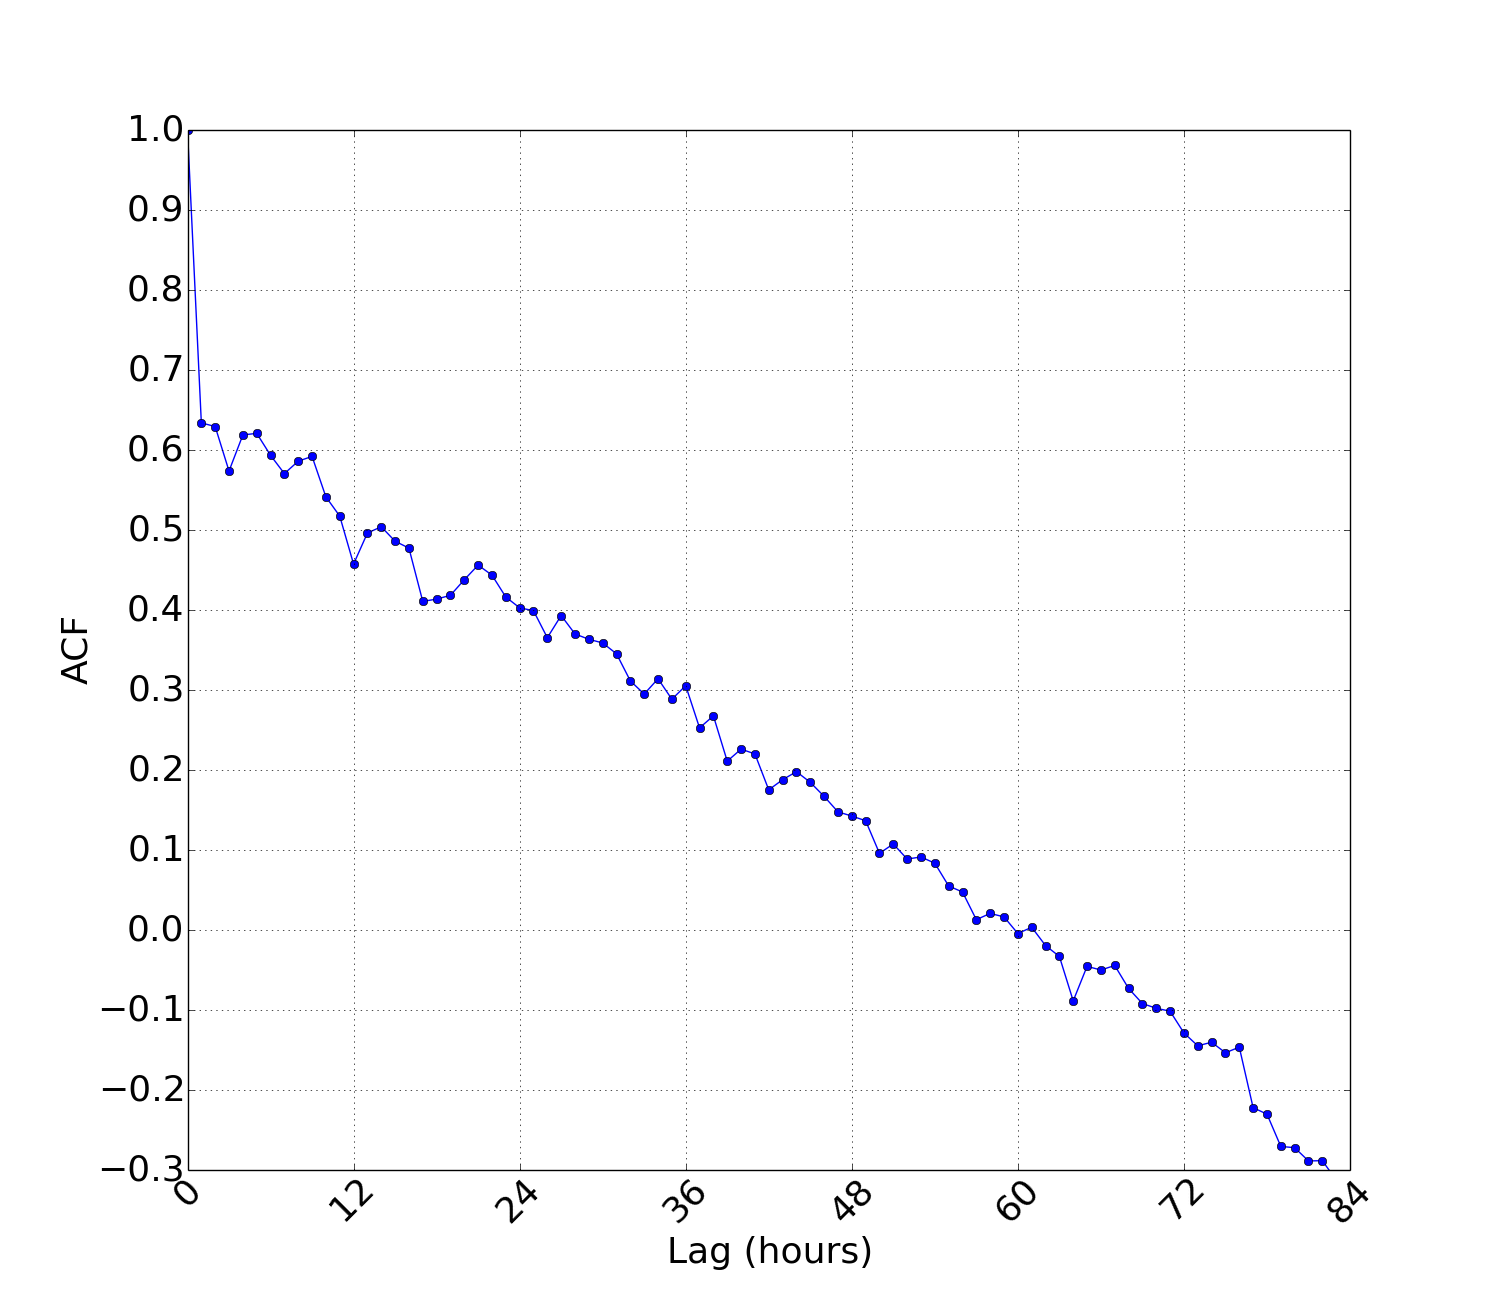
\includegraphics[width=1.0\textwidth]{./figures/acf_BHZRENPEV01_64:66:B3:A6:BA:54.png}
            \caption{Autocorrelation}
        \end{subfigure}%
        ~ 
        \begin{subfigure}[b]{0.55\textwidth}
            \centering
            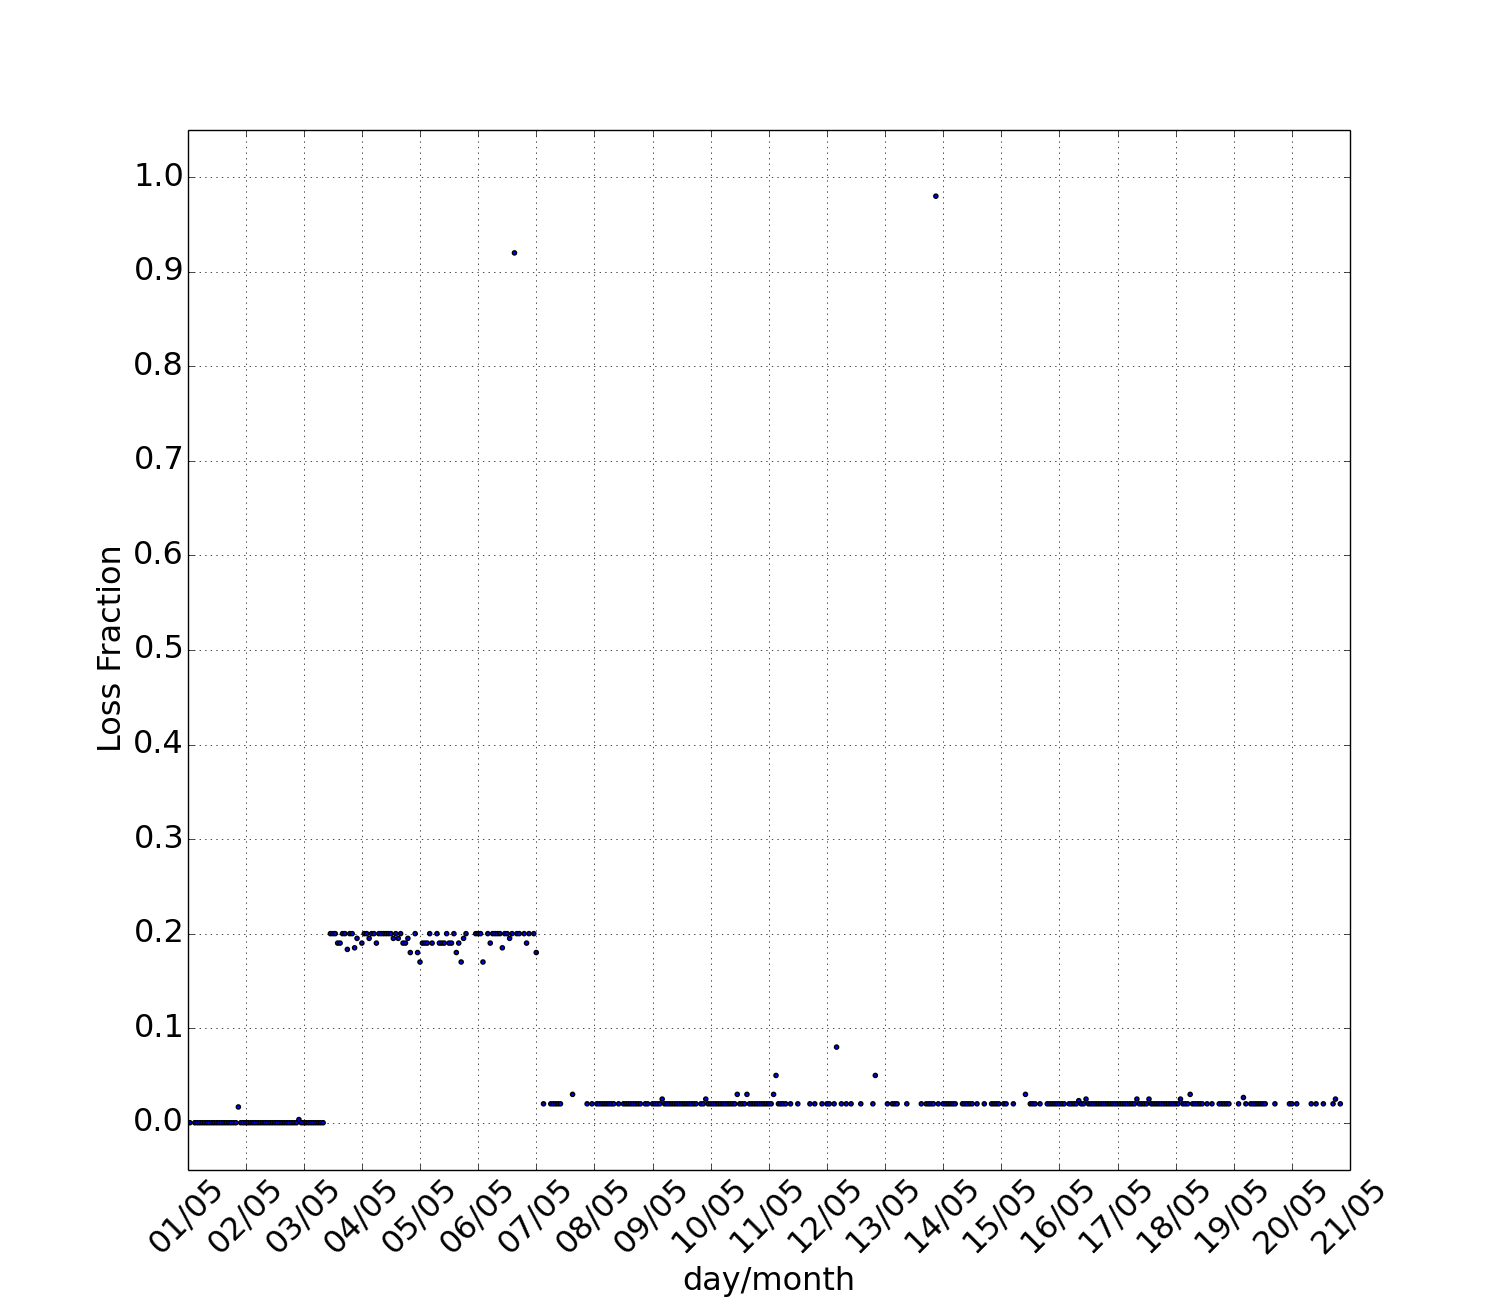
\includegraphics[width=1.0\textwidth]{./figures/ts_BHZRENPEV01_64:66:B3:A6:BA:54.png}
            \caption{Time Series}
        \end{subfigure}
    }
    \caption{Client 3}
    \label{fig:acf_ts_3}
\end{figure}

The autocorrelation of figure~\ref{fig:acf_ts_1} have a periodic pattern, with peaks in multiple of 24 hours. In this client, it is possible to observe that losses a more frequent in the end of the day. However, in figure~\ref{fig:acf_ts_2} the autocorrelation quickly decreases and fluctuates around zero. The correspondent time series have a commmon characteristics, until day 06 of may there no measures with losses, however, from then on frequently measures with losses alternated with zero losses measures. Figure~\ref{fig:acf_ts_3} shows an linear decreasing autocorrelation, and the associated time series, which presents abrupts change in the mean. 

Also, through a visual analysis, as in the previuous figures, is possible to observer diverse time series patterns and change point patterns.

As in figure~\ref{fig:acf_ts_1} same clients have a daily pattern in which losses occur more frequently at night, in which the Internet usage is known to be bigger. Figure~\ref{fig:mean_day_hour_ts} corroborates that observation, which presents the mean and variance of the measures that occurred in a specific hour during the 20 days period. This can be a indication of congestion during peak of usage hours.

\begin{figure}[H]
    \makebox[\linewidth][c]
    {
        %
        \centering
        \begin{subfigure}[b]{0.55\textwidth}
            \centering
            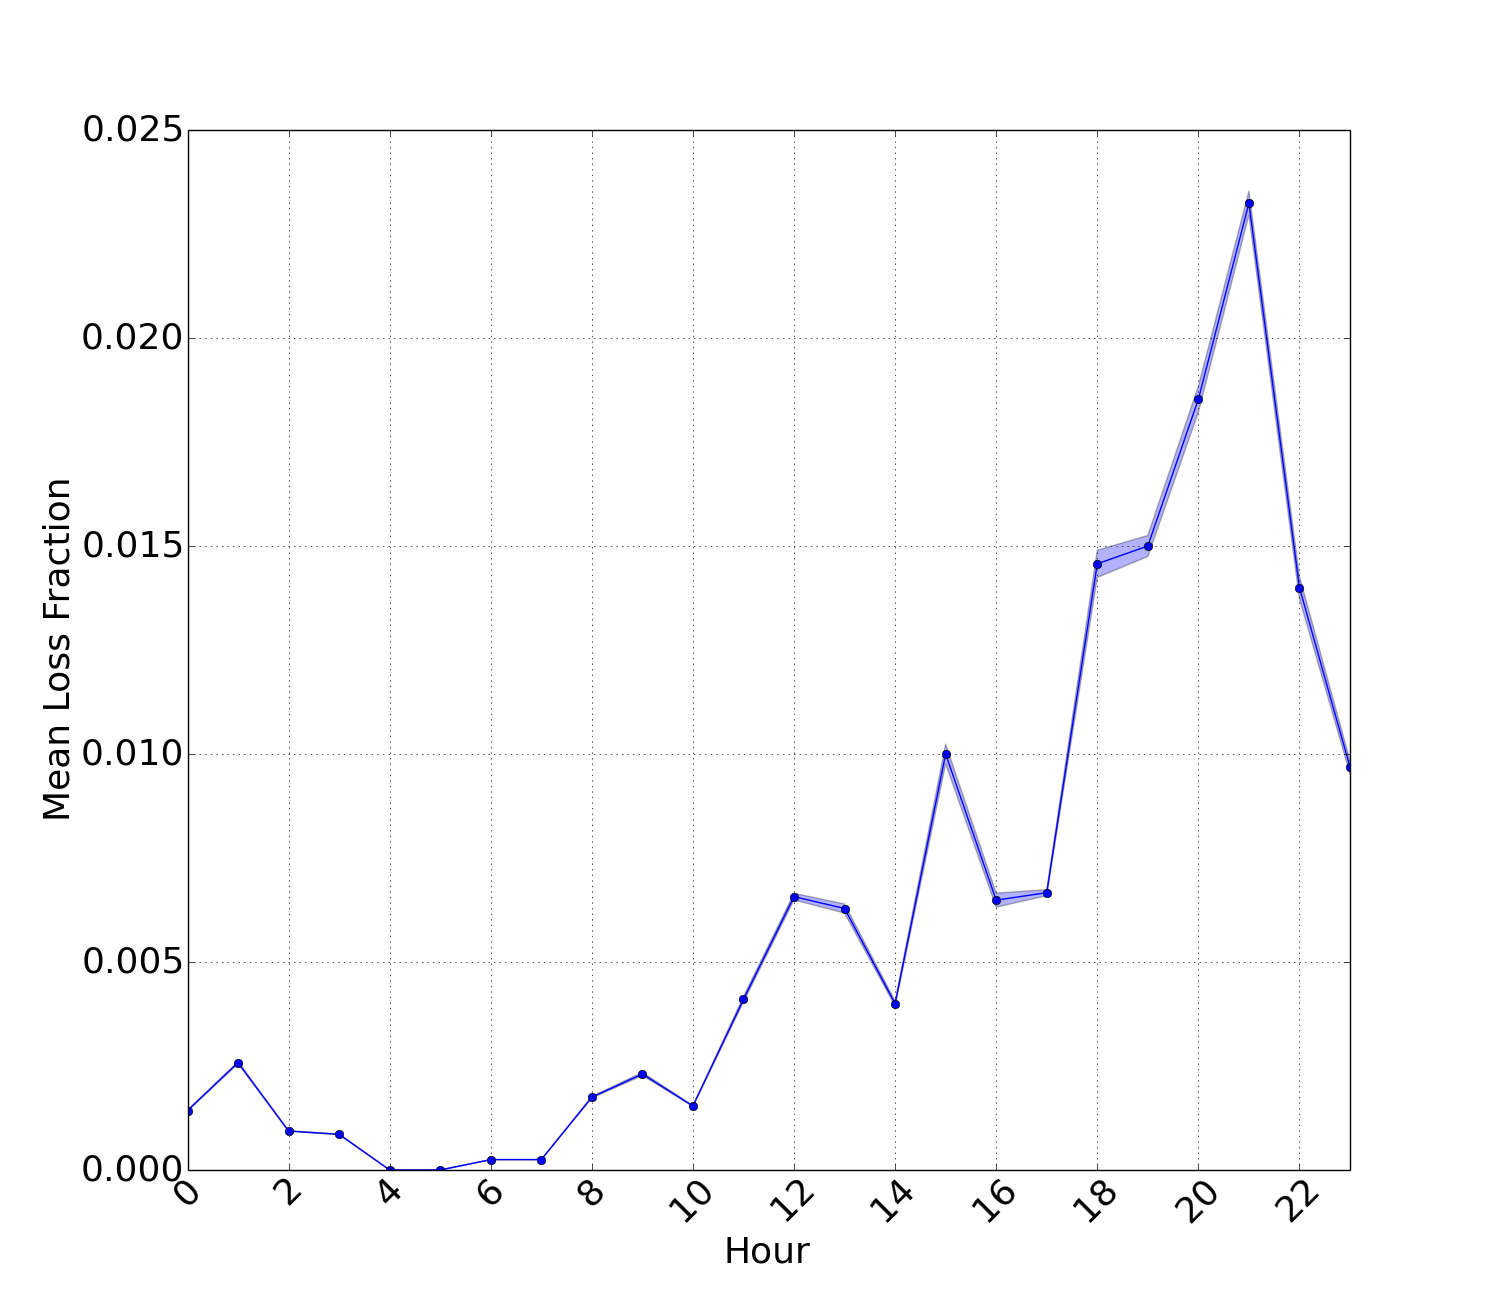
\includegraphics[width=1.0\textwidth]{./figures/mean_per_hour_in_a_day_NHODTCSRV04_64:66:B3:50:06:90.png}
            \caption{Mean and variance per hour}
        \end{subfigure}%
        ~ 
        \begin{subfigure}[b]{0.55\textwidth}
            \centering
            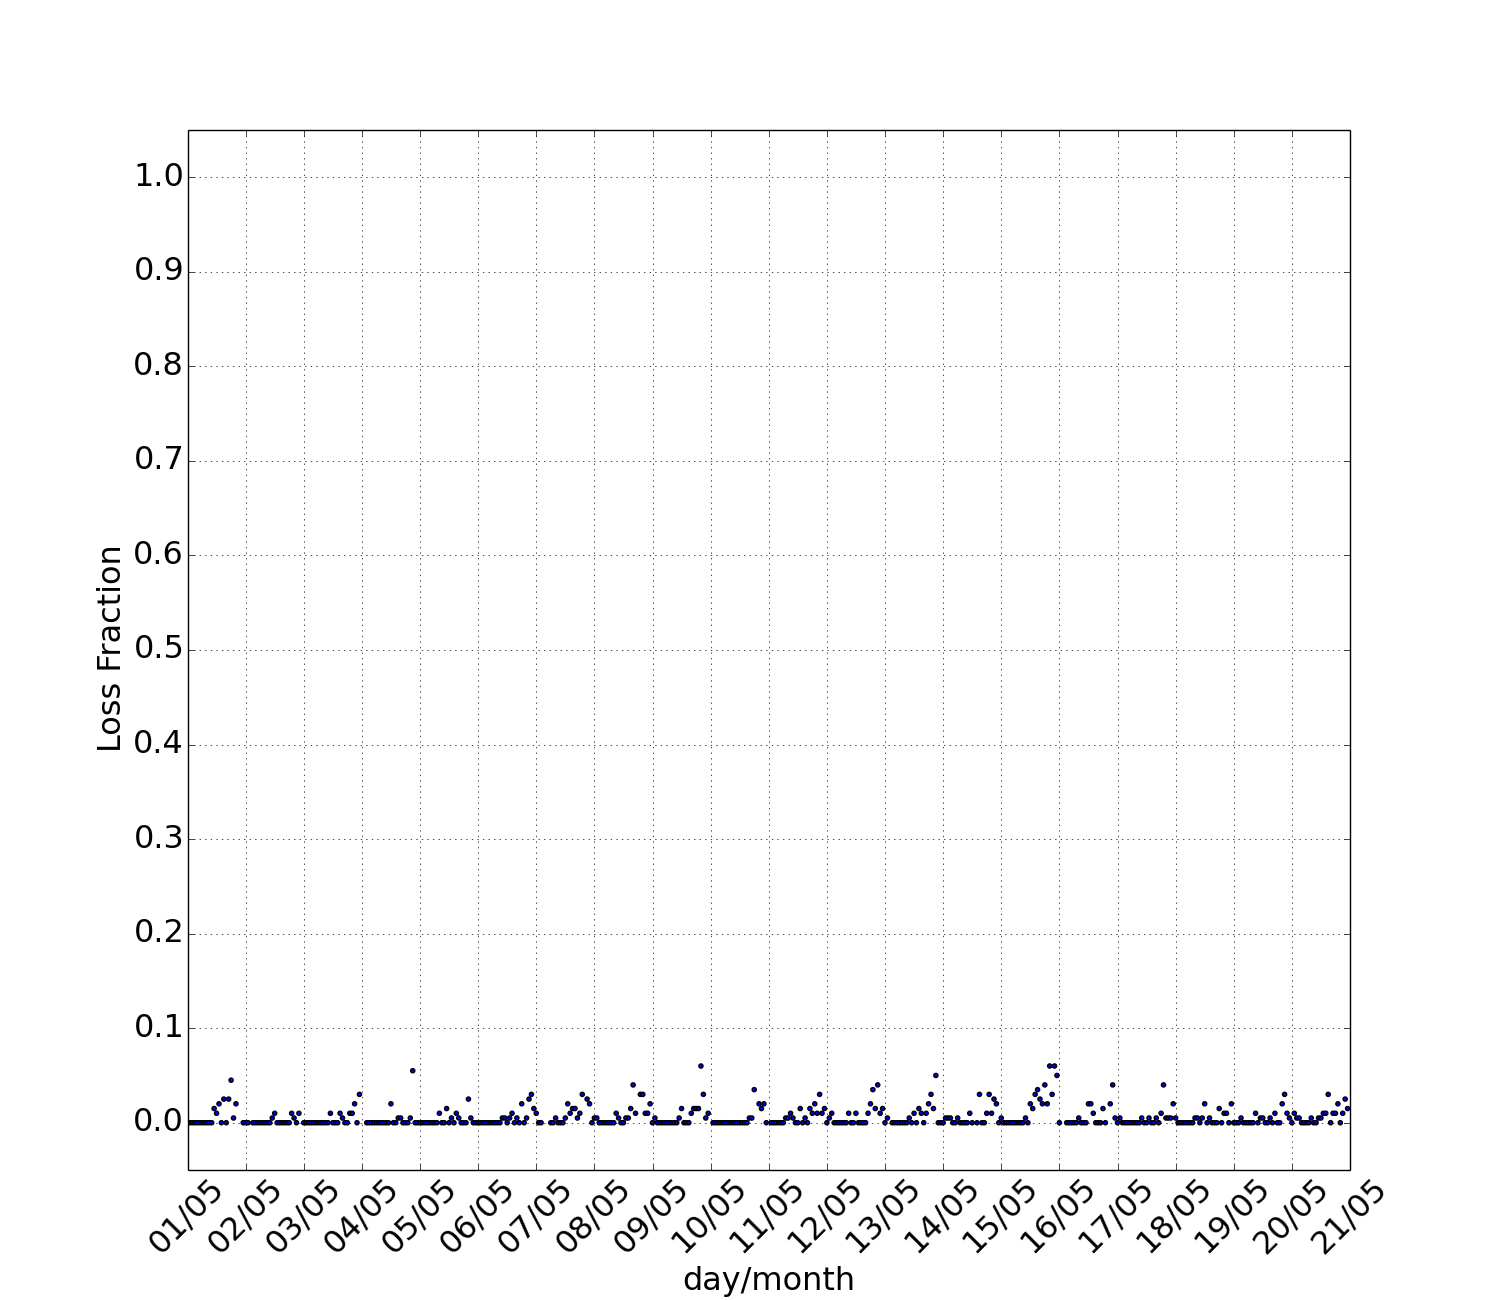
\includegraphics[width=1.0\textwidth]{./figures/ts_NHODTCSRV04_64:66:B3:50:06:90.png}
            \caption{Time Series}
        \end{subfigure}
    }
    \caption{Client 1}
    \label{fig:mean_day_hour_ts}
\end{figure}

% - mean loss by week day of single client\\
% - power spectra to check periodicity? \\

\section{Change Points Dataset}

There are several approaches to construct a change points dataset to test a change point detection method. Some works in the literature simply create a simulated time series thorugh generative models, however different segments are generated by the same model but with different parameters. In general, this types of time series are more easily handled in change point detection algorithms, since some methods assumes the same models that generated the data or because real data can have more complex characteristics. Another way is to create a time series appending different segments provenient from different real time series data. In this cases is easy to simplify the dataset since some characteristics as the segments lengths are defined by the dataset creator and another ones are fakely introduced. Another works assumes that the latent information of the time series are available, and with specific knowledge of the application field, it is possible to assume what kinds of configuration changes could induce a change in the time series. In the case of the application field of the present work this would be difficult, since the latent information would be connected with the network situation such as network topology, characteristics of routers congestions, physical equipments problems, which is a too complex, or even impossible information to collect and also to assume which variables could impact the time series. Other apprach also uses the latent information but instead creates a controlled environment in which is possible to change the configuration over time, but as in the previous case, this would be too complex. The approach followed by this work was to use a visual annotation of the time series. It were conducted, with an application domain specialist, visuallyu indicating the relevant changes. It is known that human visual inspection methods can bring erroneous conclusions, but with the data and application scenarion it was the best fit, as network engineers visually identify, after simple automatic filters, the change points.

This work is interested in work directly with real data and satisfy a real application problem.

As in other tasks, it is difficult to translate a human visual perception in a sistematically method.

In general, when the exact types of target changes are previously know the problem is easier.

\section{Methodology}

It was created an annotation system to a specialist visually indicates the change points of the time series dataset. The user indicated with the mouse the points in time where he thinks that where the cahnge points occurred. To avoid results misunderstanding X axis of the time series represented onlu the time order of the measures, since the time series are unevenly this fact could visually wrong infer change points. Also, since is known that variances in the losses fractions when the losses are low have more impact in the user QoE than when the losses are big, the system also provides two other y scales than linear, the log scale and piecewise linear with bigger length in [0, 0.1] than (0.1, 1.0]. The user can click in any scale.

A single person classified all time series. This person has experiences with academic and industry network measurements and statistical modelling, however without background in change point detection analysis. The user could take the time he wants to make a classification and it was able to classify in different days. Before the user could start the classifications, it was indicated a series of instructions: 

\begin{itemize}
    \item In the case of packet loss fraction, mean changes between 0 and 0.1 are more sensible to the end users.
    \item The "time" axis only represents the temporal order of the measurements. However, in general, consecutive points in "time" axis are separated by 30 minutes.
    \item Outlier is not a statistical change. An outlier is an observation that lies outside the overall pattern of a distribution.
\end{itemize}

Since several time series of the previously described time series have almost all measures with zero losses, these time series was filtered to reduce the number of time series and keep only the ones which provide change points, increasing the entropy. Also, to better the visualization, it was selected time with 10 days of data, therefore the dataset consists of time series from 1 may 2016 to 10 may 2016, and from 11 may 2016 to 20 may 2016. The specific filter was: it was selected only the time series that has 85\% of the maximum possible data in the specified time period, considering that each home router executes the measurement procedure at most two times in a hour. Reducing to 522 time series. Also it were only selected the time series that have at least one window of length 48 with at least 6 measures with loss fraction bigger than 0.01.

\section{Descriptive Analysis}

- explain possible ways to get the ground truth\\
- description of the volunteer\\
- user instructions\\
- snapshots of system\\ 
- how time series were selected to be in the survey\\

\section{Description of Change Points Dataset}

- number of time series, number of change points: it is a high dimensional problem\\
- distribution number of changes per time series\\
- distribution time between change points\\
- distribution time for the first change point\\
- distribution time from last change point to time series end\\
- distribution of classification time?\\
- measure the difference between consecutive segments?\\

\section{Performance Evaluation}

- how the performance is asserted in literature\\
- ROC curve\\
- confusion matrix and accuracy metrics\\

    \chapter{Conclusions}
\label{chap:conclusion}

Considering the specific \gls*{isp}'s topology, and the current end-to-end measurement
methodology, this dissertation proposes a data analytics framework to
detect and localize network events.
For such purpose, the mechanism tracks
statistical changes in the end-to-end \gls*{qos} time series from different clients,
and correlates these patterns with traceroutes.
Finally, several outcomes were presented when the procedure was applied to
real data.

The results show that, considering the exposed restrictions,
it is possible to use only end-to-end \gls*{qos} metrics, and traceroutes, from
different clients, to identify and localize network events.
However, due to the lack of an events dataset ground truth, important
questions persist unanswered.
For instance, a quantitative accuracy study
would allow to check which types of events can't be handled by the
proposed mechanism.
A dataset would also allow a precise analysis of the events
patterns, how they impact the \gls*{qos} metrics, and fine tune the system.

The use of end-to-end measurements has the advantage of dealing with
metrics that are directly related with the service perceived by the customers.
As an example, this feature can be used to rank simultaneous failure events
according with their impact to the end-users.
Nonetheless, would be interesting to study the impact of introducing
internal network information to the framework.

Besides the data availability, the current measurement process imposed
several restrictions to this work.
In order to better explore the proposed solution,
a further continuation of this project
would require a stronger partnership with the \gls*{isp}.
In addition, in order to improve the proposed framework's performance,
it would be desirable to adapt the measurement software.
However, this dissertation can be used as a first guide to the \gls*{isp}'s engineers.

\section{Contributions}
Next is summarized this dissertation contributions.

\begin{itemize}
\item
An automatic procedure, that only uses the available end-to-end \gls*{qos}
measurements, and traceroutes, to detect and localize network events in the
specific tier-3 ISP's infrastructure.

\item
A list of possible improvements in the measurement methodology currently
employed by the startup, in order to enhance the proposed system's performance. This
list is presented in the next Section~\ref{sec:future_work}.
\end{itemize}

\section{Future Work}
\label{sec:future_work}

Next is presented a list of future development directions of this work.
Considering the detection and localization of events, several adaptations to
the current measurement methodology are suggested.

\begin{itemize}
\item
The used \gls*{qos} metrics are affected by equipments in the path from the server to
the end-user, as well as those in the reverse direction.
However, only the path information from end-users to servers are available.
Hence, the traceroutes from servers to end-users should also be collected.
Besides, instead of only considering the round trip loss information,
the one way loss fraction in both directions can be tracked.
Further, the maximum achievable one way throughput measurement can be
implemented using \gls*{udp} instead of \gls*{tcp}, which eliminates the interference of
performance degradation in the reverse path.

\item
The \gls*{hfc} plant between the home router and the
first hop of the traceroute can be incorporated to the analysis.
Also, in addition to only using end-to-end \gls*{qos} metrics,
the proposed mechanism can be extended
to use internal network devices information, such as signal-to-noise ratio.

\item
A network failure events dataset can be built with \gls*{isp}'s data.
As an example, customers' complaints gathered from call centers can be used to,
during a specific time period, infer clients affected by a \gls*{qoe} deterioration,
which can then be translated to true network failures.
Additionally, it is possible to use records from current failure detection
methods deployed by the \gls*{isp}, such as manual inspection, or through equipments
that are able to report specific faults.
However, through preliminary talks with \gls*{isp}'s engineers,
both databases are noisy, and mining useful information
from them can be a challenging task.
For instance, there are cases in which devices flaws are manually
detected and corrected, but those information is not stored.
Also, during the dataset construction, the inferred events times can be
considerably different from their true occurrence time.
As stated in Chapter~\ref{chap:methodology}, a dataset could open new
supervised learning possibilities to the change point detection problem, such
as hyperparameter optimization and model selection.
Besides, since the tier-2 \gls*{isp} is not a project partner, this
complete data of the network infrastructure may not be available.

\item
Once a network events dataset is constructed, the correlation between
change points of different \gls*{qos} metrics can reveal useful information
about the network behavior. This analysis was not done since the algorithms'
hyperparameters couldn't be optimized, hence, these comparisons could reach
wrong conclusions.

\item
A deeper knowledge of the tier-2 \gls*{isp}'s infrastructure
can be used to model the tier-2 network with finer granularity in the Spatial
Correlation procedure, which can improve the system's event localization
precision.

\item
It is planned in the \gls*{isp}'s roadmap to increase the number of tracked customers.
In this case, the system's computational performance can benefit from data
aggregation techniques, as it was done in Argus.
Besides, this increase will naturally improve the internal network equipments
coverage by the end-to-end measurements, which, as the previous topic, can
enhance the events localization precision.

\item
Once the system is deployed, the algorithms and parameters can be selected
through a reinforcement learning approach. If network operators
feedback the outcomes' correctness, the system can adaptively optimize the used
strategies.

\item
Considering a real time processing environment, in order to decrease the
event detection delay, the system can adaptively control the measurement
frequency.
Increasing the amount of data related to potentially problematic regions,
can improve the system's output confidence in a short time period.
Also, it is possible to reduce the measurement frequency in well behaved
localities, which can lower the traffic overhead generated by measurements, and
increase the data analytics computational performance.

\item
Instead of centrally process the time series,
it is possible to instrument the home
gateways to detect changes in an online fashion. Then, as with \gls*{cem}, the home
routers could push this information to a central database for further analysis.

\item
Extend the mechanism to deal with other types of network infrastructures.

\end{itemize}

    
    \backmatter
    \nocite{*}
    \bibliographystyle{coppe-unsrt}
    \bibliography{./src/bibliography}

\end{document}
